% Preamble
% ---
\documentclass{article}
\parindent0pt
\newcommand{\forceindent}{\leavevmode{\parindent=3em\indent}}

% Packages
% ---
\usepackage{amsmath}
\usepackage{graphicx}

\begin{document}

	\title{Electronics Equations}
	\author{Tyler Hilbert}
	\date{}
	\maketitle

	\subsection*{Electronic Formula Wheel}
	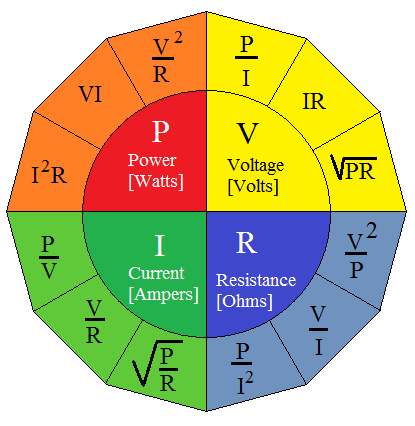
\includegraphics[width=50mm]{FormulaWheel.png}

	\section*{Equations from ``Fundamentals of Electric Circuits''}
	% TODO - double check for all equations in chapter 1&2

	Current: $I = dQ/dt$ \\*[\smallskipamount]
	\forceindent (Note: This can also be written like this: $I = \Delta Q / \Delta t$)
	
	Charge: $Q = \int_{to}^{t} i\,dt$

	Voltage: $V = dw/dQ$

	Power: $p = dw/dt$
	
	
	Kirchoff's Law: $\sum\limits_{m=1}^{M} v_{m} = 0$ 
	
	Resistance in series: $\sum\limits_{n=1}^{N} R_{n}$
	
	Resistance in parallel: $R = 1/\sum\limits_{n=1}^{N} 1/R_{n}$
	
	\section*{Delta Wye conversion}
	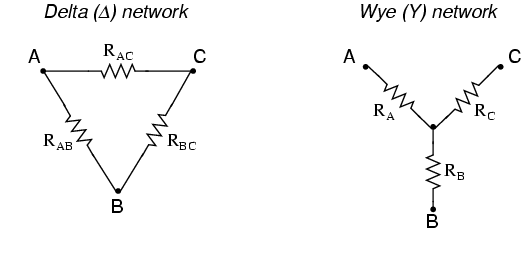
\includegraphics[width=80mm]{DeltaWye.png}
	
	Delta($\Delta$) to Wye(Y): $R_{A} = \dfrac{R_{AB}R_{AC}}{R_{AB}+R_{AC}+R{BC}}$
	
	Wye(Y) to Delta($\Delta$): $R_{AB} = \dfrac{R_{A}R_{B} + R_{A}R_{C} + R_{B}R_{C}} {R_{C}} $

	
	
	% TODO - add references

\end{document}